%%
% Copyright (c) 2017 - 2019, Pascal Wagler;  
% Copyright (c) 2014 - 2019, John MacFarlane
% 
% All rights reserved.
% 
% Redistribution and use in source and binary forms, with or without 
% modification, are permitted provided that the following conditions 
% are met:
% 
% - Redistributions of source code must retain the above copyright 
% notice, this list of conditions and the following disclaimer.
% 
% - Redistributions in binary form must reproduce the above copyright 
% notice, this list of conditions and the following disclaimer in the 
% documentation and/or other materials provided with the distribution.
% 
% - Neither the name of John MacFarlane nor the names of other 
% contributors may be used to endorse or promote products derived 
% from this software without specific prior written permission.
% 
% THIS SOFTWARE IS PROVIDED BY THE COPYRIGHT HOLDERS AND CONTRIBUTORS 
% "AS IS" AND ANY EXPRESS OR IMPLIED WARRANTIES, INCLUDING, BUT NOT 
% LIMITED TO, THE IMPLIED WARRANTIES OF MERCHANTABILITY AND FITNESS 
% FOR A PARTICULAR PURPOSE ARE DISCLAIMED. IN NO EVENT SHALL THE 
% COPYRIGHT OWNER OR CONTRIBUTORS BE LIABLE FOR ANY DIRECT, INDIRECT, 
% INCIDENTAL, SPECIAL, EXEMPLARY, OR CONSEQUENTIAL DAMAGES (INCLUDING,
% BUT NOT LIMITED TO, PROCUREMENT OF SUBSTITUTE GOODS OR SERVICES; 
% LOSS OF USE, DATA, OR PROFITS; OR BUSINESS INTERRUPTION) HOWEVER 
% CAUSED AND ON ANY THEORY OF LIABILITY, WHETHER IN CONTRACT, STRICT 
% LIABILITY, OR TORT (INCLUDING NEGLIGENCE OR OTHERWISE) ARISING IN 
% ANY WAY OUT OF THE USE OF THIS SOFTWARE, EVEN IF ADVISED OF THE 
% POSSIBILITY OF SUCH DAMAGE.
%%

%%
% This is the Eisvogel pandoc LaTeX template.
%
% For usage information and examples visit the official GitHub page:
% https://github.com/Wandmalfarbe/pandoc-latex-template
%%

\PassOptionsToPackage{unicode=true}{hyperref} % options for packages loaded elsewhere
\PassOptionsToPackage{hyphens}{url}
\PassOptionsToPackage{dvipsnames,svgnames*,x11names*,table}{xcolor}
%
\documentclass[
  10pt,
  english,
  letterpaper,
,tablecaptionabove
]{scrartcl}
\usepackage{lmodern}
\usepackage{setspace}
\setstretch{1.2}
\usepackage{amssymb,amsmath}
\usepackage{ifxetex,ifluatex}
\ifnum 0\ifxetex 1\fi\ifluatex 1\fi=0 % if pdftex
  \usepackage[T1]{fontenc}
  \usepackage[utf8]{inputenc}
  \usepackage{textcomp} % provides euro and other symbols
\else % if luatex or xelatex
  \usepackage{unicode-math}
  \defaultfontfeatures{Scale=MatchLowercase}
  \defaultfontfeatures[\rmfamily]{Ligatures=TeX,Scale=1}
\fi
% use upquote if available, for straight quotes in verbatim environments
\IfFileExists{upquote.sty}{\usepackage{upquote}}{}
\IfFileExists{microtype.sty}{% use microtype if available
  \usepackage[]{microtype}
  \UseMicrotypeSet[protrusion]{basicmath} % disable protrusion for tt fonts
}{}
\makeatletter
\@ifundefined{KOMAClassName}{% if non-KOMA class
  \IfFileExists{parskip.sty}{%
    \usepackage{parskip}
  }{% else
    \setlength{\parindent}{0pt}
    \setlength{\parskip}{6pt plus 2pt minus 1pt}}
}{% if KOMA class
  \KOMAoptions{parskip=half}}
\makeatother
\usepackage{xcolor}
\definecolor{default-linkcolor}{HTML}{A50000}
\definecolor{default-filecolor}{HTML}{A50000}
\definecolor{default-citecolor}{HTML}{4077C0}
\definecolor{default-urlcolor}{HTML}{4077C0}
\IfFileExists{xurl.sty}{\usepackage{xurl}}{} % add URL line breaks if available
\IfFileExists{bookmark.sty}{\usepackage{bookmark}}{\usepackage{hyperref}}
\hypersetup{
  pdftitle={Graphs (Part 3)},
  pdfauthor={Connor Baker},
  pdfsubject={Graphs},
  pdfkeywords={Lecture, Graphs},
  pdfborder={0 0 0},
  breaklinks=true}
\urlstyle{same}  % don't use monospace font for urls
\usepackage[margin=2.5cm,includehead=true,includefoot=true,centering]{geometry}
\usepackage{listings}
\newcommand{\passthrough}[1]{#1}
\lstset{defaultdialect=[5.3]Lua}
\lstset{defaultdialect=[x86masm]Assembler}
\usepackage{longtable,booktabs}
% Allow footnotes in longtable head/foot
\IfFileExists{footnotehyper.sty}{\usepackage{footnotehyper}}{\usepackage{footnote}}
\makesavenoteenv{longtable}
\usepackage{graphicx,grffile}
\makeatletter
\def\maxwidth{\ifdim\Gin@nat@width>\linewidth\linewidth\else\Gin@nat@width\fi}
\def\maxheight{\ifdim\Gin@nat@height>\textheight\textheight\else\Gin@nat@height\fi}
\makeatother
% Scale images if necessary, so that they will not overflow the page
% margins by default, and it is still possible to overwrite the defaults
% using explicit options in \includegraphics[width, height, ...]{}
\setkeys{Gin}{width=\maxwidth,height=\maxheight,keepaspectratio}
\usepackage[normalem]{ulem}
% avoid problems with \sout in headers with hyperref:
\pdfstringdefDisableCommands{\renewcommand{\sout}{}}
\setlength{\emergencystretch}{3em}  % prevent overfull lines
\providecommand{\tightlist}{%
  \setlength{\itemsep}{0pt}\setlength{\parskip}{0pt}}
\setcounter{secnumdepth}{-\maxdimen} % remove section numbering
% Redefines (sub)paragraphs to behave more like sections
\ifx\paragraph\undefined\else
  \let\oldparagraph\paragraph
  \renewcommand{\paragraph}[1]{\oldparagraph{#1}\mbox{}}
\fi
\ifx\subparagraph\undefined\else
  \let\oldsubparagraph\subparagraph
  \renewcommand{\subparagraph}[1]{\oldsubparagraph{#1}\mbox{}}
\fi

% Make use of float-package and set default placement for figures to H
\usepackage{float}
\floatplacement{figure}{H}

\setcounter{page}{0}
\lstset{breaklines=true}
\lstset{postbreak=\raisebox{0ex}[0ex][0ex]{\ensuremath{\color{blue}\hookrightarrow\space}}}
\usepackage{datetime}
\settimeformat{ampmtime}
\usepackage{lastpage}
\ifnum 0\ifxetex 1\fi=0 % if pdftex or luatex
  \usepackage[shorthands=off,main=english]{babel}
\else % if xetex
    % See issue https://github.com/reutenauer/polyglossia/issues/127
  \renewcommand*\familydefault{\sfdefault}
    % load polyglossia as late as possible as it *could* call bidi if RTL lang (e.g. Hebrew or Arabic)
  \usepackage{polyglossia}
  \setmainlanguage[]{english}
\fi

\title{Graphs (Part 3)}
\usepackage{etoolbox}
\makeatletter
\providecommand{\subtitle}[1]{% add subtitle to \maketitle
  \apptocmd{\@title}{\par {\large #1 \par}}{}{}
}
\makeatother
\subtitle{Graph traversals, the shortest path problem, and the minimum spanning
tree problem}
\author{Connor Baker}
\date{2019-03-28, Compiled on \today~at \currenttime}





%%
%% added
%%

%
% language specification
%
% If no language is specified, use English as the default main document language.
%


%
% for the background color of the title page
%
\usepackage{pagecolor}
\usepackage{afterpage}

%
% TOC depth and 
% section numbering depth
%
\setcounter{tocdepth}{3}

%
% break urls
%
\PassOptionsToPackage{hyphens}{url}

%
% When using babel or polyglossia with biblatex, loading csquotes is recommended 
% to ensure that quoted texts are typeset according to the rules of your main language.
%
\usepackage{csquotes}

%
% captions
%
\definecolor{caption-color}{HTML}{777777}
\usepackage[font={stretch=1.2}, textfont={color=caption-color}, position=top, skip=4mm, labelfont=bf, singlelinecheck=false, justification=raggedright]{caption}
\setcapindent{0em}

%
% blockquote
%
\definecolor{blockquote-border}{RGB}{221,221,221}
\definecolor{blockquote-text}{RGB}{119,119,119}
\usepackage{mdframed}
\newmdenv[rightline=false,bottomline=false,topline=false,linewidth=3pt,linecolor=blockquote-border,skipabove=\parskip]{customblockquote}
\renewenvironment{quote}{\begin{customblockquote}\list{}{\rightmargin=0em\leftmargin=0em}%
\item\relax\color{blockquote-text}\ignorespaces}{\unskip\unskip\endlist\end{customblockquote}}

%
% Source Sans Pro as the de­fault font fam­ily
% Source Code Pro for monospace text
%
% 'default' option sets the default 
% font family to Source Sans Pro, not \sfdefault.
%
\usepackage[default]{sourcesanspro}
\usepackage{sourcecodepro}

% XeLaTeX specific adjustments for straight quotes: https://tex.stackexchange.com/a/354887
% This issue is already fixed (see https://github.com/silkeh/latex-sourcecodepro/pull/5) but the 
% fix is still unreleased.
% TODO: Remove this workaround when the new version of sourcecodepro is released on CTAN.
\ifxetex
\makeatletter
\defaultfontfeatures[\ttfamily]
  { Numbers   = \sourcecodepro@figurestyle,
    Scale     = \SourceCodePro@scale,
    Extension = .otf }
\setmonofont
  [ UprightFont    = *-\sourcecodepro@regstyle,
    ItalicFont     = *-\sourcecodepro@regstyle It,
    BoldFont       = *-\sourcecodepro@boldstyle,
    BoldItalicFont = *-\sourcecodepro@boldstyle It ]
  {SourceCodePro}
\makeatother
\fi

%
% heading color
%
\definecolor{heading-color}{RGB}{40,40,40}
\addtokomafont{section}{\color{heading-color}}
% When using the classes report, scrreprt, book, 
% scrbook or memoir, uncomment the following line.
%\addtokomafont{chapter}{\color{heading-color}}

%
% variables for title and author
%
\usepackage{titling}
\title{Graphs (Part 3)}
\author{Connor Baker}

%
% tables
%

\definecolor{table-row-color}{HTML}{F5F5F5}
\definecolor{table-rule-color}{HTML}{999999}

%\arrayrulecolor{black!40}
\arrayrulecolor{table-rule-color}     % color of \toprule, \midrule, \bottomrule
\setlength\heavyrulewidth{0.3ex}      % thickness of \toprule, \bottomrule
\renewcommand{\arraystretch}{1.3}     % spacing (padding)

% Reset rownum counter so that each table
% starts with the same row colors.
% https://tex.stackexchange.com/questions/170637/restarting-rowcolors
\let\oldlongtable\longtable
\let\endoldlongtable\endlongtable
\renewenvironment{longtable}{
\rowcolors{3}{}{table-row-color!100}  % row color
\oldlongtable} {
\endoldlongtable
\global\rownum=0\relax}

% Unfortunately the colored cells extend beyond the edge of the 
% table because pandoc uses @-expressions (@{}) like so: 
%
% \begin{longtable}[]{@{}ll@{}}
% \end{longtable}
%
% https://en.wikibooks.org/wiki/LaTeX/Tables#.40-expressions

%
% remove paragraph indention
%
\setlength{\parindent}{0pt}
\setlength{\parskip}{6pt plus 2pt minus 1pt}
\setlength{\emergencystretch}{3em}  % prevent overfull lines

%
%
% Listings
%
%


%
% listing colors
%
\definecolor{listing-background}{HTML}{F7F7F7}
\definecolor{listing-rule}{HTML}{B3B2B3}
\definecolor{listing-numbers}{HTML}{B3B2B3}
\definecolor{listing-text-color}{HTML}{000000}
\definecolor{listing-keyword}{HTML}{435489}
\definecolor{listing-identifier}{HTML}{435489}
\definecolor{listing-string}{HTML}{00999A}
\definecolor{listing-comment}{HTML}{8E8E8E}
\definecolor{listing-javadoc-comment}{HTML}{006CA9}

\lstdefinestyle{eisvogel_listing_style}{
  language         = java,
  numbers          = left,
  xleftmargin      = 2.7em,
  framexleftmargin = 2.5em,
  backgroundcolor  = \color{listing-background},
  basicstyle       = \color{listing-text-color}\small\ttfamily{}\linespread{1.15}, % print whole listing small
  breaklines       = true,
  frame            = single,
  framesep         = 0.19em,
  rulecolor        = \color{listing-rule},
  frameround       = ffff,
  tabsize          = 4,
  numberstyle      = \color{listing-numbers},
  aboveskip        = -0.7em,
  belowskip        = 0.1em,
  abovecaptionskip = 0em,
  belowcaptionskip = 1em,
  keywordstyle     = \color{listing-keyword}\bfseries,
  classoffset      = 0,
  sensitive        = true,
  identifierstyle  = \color{listing-identifier},
  commentstyle     = \color{listing-comment},
  morecomment      = [s][\color{listing-javadoc-comment}]{/**}{*/},
  stringstyle      = \color{listing-string},
  showstringspaces = false,
  escapeinside     = {/*@}{@*/}, % Allow LaTeX inside these special comments
  literate         =
  {á}{{\'a}}1 {é}{{\'e}}1 {í}{{\'i}}1 {ó}{{\'o}}1 {ú}{{\'u}}1
  {Á}{{\'A}}1 {É}{{\'E}}1 {Í}{{\'I}}1 {Ó}{{\'O}}1 {Ú}{{\'U}}1
  {à}{{\`a}}1 {è}{{\'e}}1 {ì}{{\`i}}1 {ò}{{\`o}}1 {ù}{{\`u}}1
  {À}{{\`A}}1 {È}{{\'E}}1 {Ì}{{\`I}}1 {Ò}{{\`O}}1 {Ù}{{\`U}}1
  {ä}{{\"a}}1 {ë}{{\"e}}1 {ï}{{\"i}}1 {ö}{{\"o}}1 {ü}{{\"u}}1
  {Ä}{{\"A}}1 {Ë}{{\"E}}1 {Ï}{{\"I}}1 {Ö}{{\"O}}1 {Ü}{{\"U}}1
  {â}{{\^a}}1 {ê}{{\^e}}1 {î}{{\^i}}1 {ô}{{\^o}}1 {û}{{\^u}}1
  {Â}{{\^A}}1 {Ê}{{\^E}}1 {Î}{{\^I}}1 {Ô}{{\^O}}1 {Û}{{\^U}}1
  {œ}{{\oe}}1 {Œ}{{\OE}}1 {æ}{{\ae}}1 {Æ}{{\AE}}1 {ß}{{\ss}}1
  {ç}{{\c c}}1 {Ç}{{\c C}}1 {ø}{{\o}}1 {å}{{\r a}}1 {Å}{{\r A}}1
  {€}{{\EUR}}1 {£}{{\pounds}}1 {«}{{\guillemotleft}}1
  {»}{{\guillemotright}}1 {ñ}{{\~n}}1 {Ñ}{{\~N}}1 {¿}{{?`}}1
  {…}{{\ldots}}1 {≥}{{>=}}1 {≤}{{<=}}1 {„}{{\glqq}}1 {“}{{\grqq}}1
  {”}{{''}}1
}
\lstset{style=eisvogel_listing_style}

\lstdefinelanguage{XML}{
  morestring      = [b]",
  moredelim       = [s][\bfseries\color{listing-keyword}]{<}{\ },
  moredelim       = [s][\bfseries\color{listing-keyword}]{</}{>},
  moredelim       = [l][\bfseries\color{listing-keyword}]{/>},
  moredelim       = [l][\bfseries\color{listing-keyword}]{>},
  morecomment     = [s]{<?}{?>},
  morecomment     = [s]{<!--}{-->},
  commentstyle    = \color{listing-comment},
  stringstyle     = \color{listing-string},
  identifierstyle = \color{listing-identifier}
}

%
% header and footer
%
\usepackage{fancyhdr}

\fancypagestyle{eisvogel-header-footer}{
  \fancyhead{}
  \fancyfoot{}
  \lhead[2019-03-28]{Graphs (Part 3)}
  \chead[]{}
  \rhead[Graphs (Part 3)]{2019-03-28}
  \lfoot[\thepage~of \pageref{LastPage}]{Connor Baker}
  \cfoot[]{}
  \rfoot[Connor Baker]{\thepage~of \pageref{LastPage}}
  \renewcommand{\headrulewidth}{0.4pt}
  \renewcommand{\footrulewidth}{0.4pt}
}
\pagestyle{eisvogel-header-footer}

%%
%% end added
%%

\begin{document}

%%
%% begin titlepage
%%

\begin{titlepage}
\newgeometry{left=6cm}
\definecolor{titlepage-color}{HTML}{FFFFFF}
\newpagecolor{titlepage-color}\afterpage{\restorepagecolor}
\newcommand{\colorRule}[3][black]{\textcolor[HTML]{#1}{\rule{#2}{#3}}}
\begin{flushleft}
\noindent
\\[-1em]
\color[HTML]{0d47a1}
\makebox[0pt][l]{\colorRule[0d47a1]{1.3\textwidth}{2pt}}
\par
\noindent

{ \setstretch{1.4}
\vfill
\noindent {\huge \textbf{\textsf{Graphs (Part 3)}}}
\vskip 1em
{\Large \textsf{Graph traversals, the shortest path problem, and the minimum spanning
tree problem}}
\vskip 2em
\noindent
{\Large \textsf{Connor Baker}
\vfill
}


\textsf{2019-03-28, Compiled on \today~at \currenttime}}
\end{flushleft}
\end{titlepage}
\restoregeometry

%%
%% end titlepage
%%



\hypertarget{graphs-part-3}{%
\section{Graphs (Part 3)}\label{graphs-part-3}}

\hypertarget{positive-weighted-shortest-path}{%
\subsection{Positive Weighted Shortest
Path}\label{positive-weighted-shortest-path}}

\begin{itemize}
\item
  Weighted graph

  \begin{itemize}
  \tightlist
  \item
    A path with fewer edges may not have a lower cost, since each edge
    carries its own weight
  \item
    We must calculate and compare the total weight
  \end{itemize}
\item
  Example:

  \begin{figure}
  \centering
  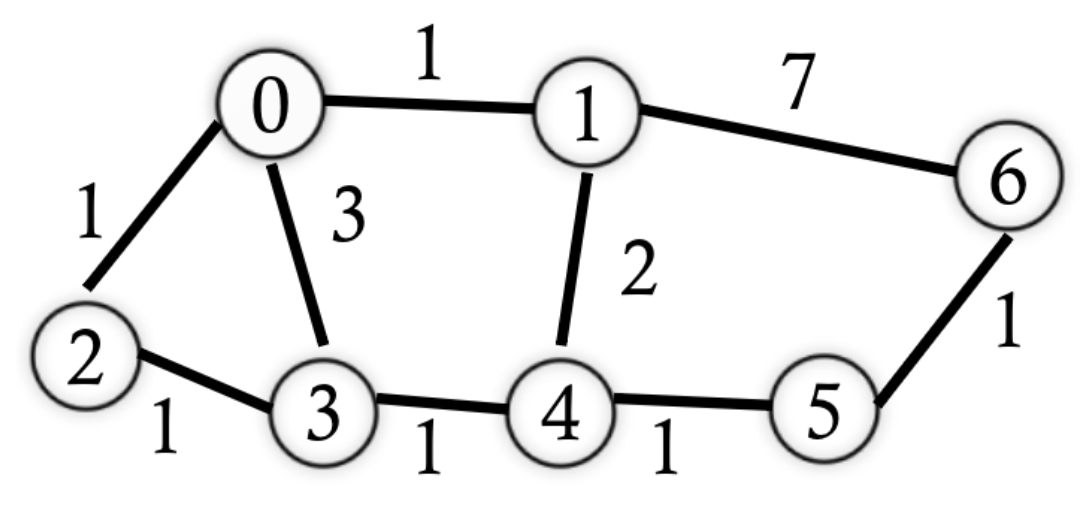
\includegraphics[width=0.5\textwidth,height=\textheight]{images/1.png}
  \caption{Example 1}
  \end{figure}

  \begin{itemize}
  \tightlist
  \item
    What's the shortest path from \(0\) to \(6\)?

    \begin{itemize}
    \tightlist
    \item
      Shortest in terms of edges:

      \begin{itemize}
      \tightlist
      \item
        The path \(\{0, 1, 6\}\) with weight \(8\)
      \end{itemize}
    \item
      Shortest in terms of weight:

      \begin{itemize}
      \tightlist
      \item
        The path \(\{0, 1, 4 ,5, 6\}\) with weight \(5\)
      \end{itemize}
    \end{itemize}
  \end{itemize}
\item
  As a general solution, we can use \emph{Dijkstra's Algorithm}

  \begin{itemize}
  \tightlist
  \item
    We don't allow negative edges
  \item
    Each node remembers the current shortest path (the previous path and
    the distance)

    \begin{itemize}
    \tightlist
    \item
      All nodes start at \(\infty\), except for the starting node \(S\)
    \end{itemize}
  \item
    Repeat the following until all nodes have been marked:

    \begin{itemize}
    \tightlist
    \item
      Take the node \(m\) which has the minimum distance among all nodes
      that have not been marked and mark it
    \item
      Update the unmarked nodes connected to node \(m\) if the path via
      \(m\) is shorter
    \end{itemize}
  \end{itemize}
\end{itemize}

\hypertarget{example-of-dijkstras-algorithm}{%
\subsection{Example of Dijkstra's
Algorithm}\label{example-of-dijkstras-algorithm}}

Suppose we want to find the shortest path given the following graph, and
starting at vertex \(0\).

\begin{figure}
\centering
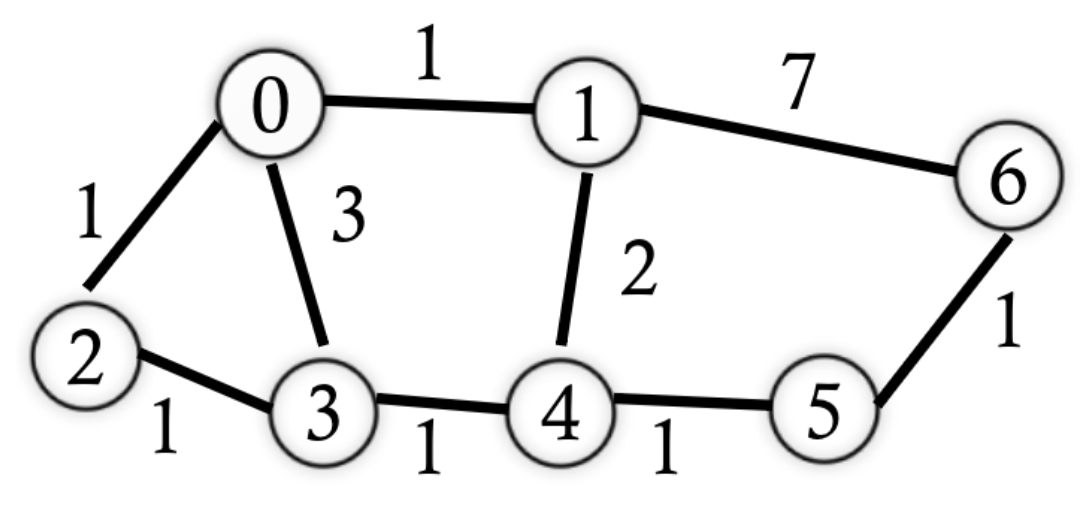
\includegraphics[width=0.5\textwidth,height=\textheight]{images/1.png}
\caption{Example 2}
\end{figure}

\begin{longtable}[]{cccccccc}
\toprule
Node & 0 & 1 & 2 & 3 & 4 & 5 & 6\tabularnewline
\midrule
\endhead
Path Length & 0 & \(\infty\) & \(\infty\) & \(\infty\) & \(\infty\) &
\(\infty\) & \(\infty\)\tabularnewline
Prev & 0 & - & - & - & - & - & -\tabularnewline
\bottomrule
\end{longtable}

\begin{itemize}
\tightlist
\item
  Starting vertex \(0\)

  \begin{itemize}
  \tightlist
  \item
    Updating for vertices \(1\), \(2\), and \(3\)
  \end{itemize}
\item
  Paths: \(\{\}\)
\end{itemize}

\begin{longtable}[]{cccccccc}
\toprule
Node & 0 & 1 & 2 & 3 & 4 & 5 & 6\tabularnewline
\midrule
\endhead
Path Length & 0 & 1 & 1 & 3 & \(\infty\) & \(\infty\) &
\(\infty\)\tabularnewline
Prev & 0 & 0 & 0 & 0 & - & - & -\tabularnewline
\bottomrule
\end{longtable}

\begin{itemize}
\tightlist
\item
  Next vertex \(1\)

  \begin{itemize}
  \tightlist
  \item
    Updating for vertices \(4\) and \(6\)
  \end{itemize}
\item
  Paths: \(\{0, 1\}\)
\end{itemize}

\begin{longtable}[]{cccccccc}
\toprule
Node & 0 & 1 & 2 & 3 & 4 & 5 & 6\tabularnewline
\midrule
\endhead
Path Length & 0 & 1 & 1 & 3 & 3 & \(\infty\) & 8\tabularnewline
Prev & 0 & 0 & 0 & 0 & 1 & - & 1\tabularnewline
\bottomrule
\end{longtable}

\begin{itemize}
\tightlist
\item
  Next vertex \(2\)

  \begin{itemize}
  \tightlist
  \item
    Updating for vertex \(3\)
  \end{itemize}
\item
  Paths: \(\{0, 1\}, \{0, 2\}\)
\end{itemize}

\begin{longtable}[]{cccccccc}
\toprule
Node & 0 & 1 & 2 & 3 & 4 & 5 & 6\tabularnewline
\midrule
\endhead
Path Length & 0 & 1 & 1 & \sout{3} 2 & 3 & \(\infty\) & 8\tabularnewline
Prev & 0 & 0 & 0 & \sout{0} 2 & 1 & - & 1\tabularnewline
\bottomrule
\end{longtable}

\begin{itemize}
\tightlist
\item
  Next vertex \(3\)

  \begin{itemize}
  \tightlist
  \item
    Updating for vertex \(3\)

    \begin{itemize}
    \tightlist
    \item
      Reached every node, update nothing
    \end{itemize}
  \end{itemize}
\item
  Paths: \(\{0, 1\}, \{0, 2\}, \{0, 2, 3\}\)
\end{itemize}

\begin{longtable}[]{cccccccc}
\toprule
Node & 0 & 1 & 2 & 3 & 4 & 5 & 6\tabularnewline
\midrule
\endhead
Path Length & 0 & 1 & 1 & \sout{3} 2 & 3 & 4 & \sout{8} 5\tabularnewline
Prev & 0 & 0 & 0 & \sout{0} 2 & 1 & 4 & \sout{1} 5\tabularnewline
\bottomrule
\end{longtable}

\begin{itemize}
\tightlist
\item
  Next vertex \(4\)

  \begin{itemize}
  \tightlist
  \item
    Updating for vertex \(5\)
  \end{itemize}
\item
  Paths:
  \(\{0, 1\}, \{0, 2\}, \{0, 2, 3\}, \{0, 1, 4\}, \{0, 1, 4, 5\}, \{0, 1, 4, 5, 6\}\)
\end{itemize}

Our final record is then

\begin{longtable}[]{cccccccc}
\toprule
Node & 0 & 1 & 2 & 3 & 4 & 5 & 6\tabularnewline
\midrule
\endhead
Path Length & 0 & 1 & 1 & \sout{3} 2 & 3 & 4 & \sout{8} 5\tabularnewline
Prev & 0 & 0 & 0 & \sout{0} 2 & 1 & 4 & \sout{1} 5\tabularnewline
\bottomrule
\end{longtable}

\begin{itemize}
\tightlist
\item
  Prev: the previous node in the shortest path starting from \(0\)
\item
  Path length: length of the corresponding shortest path
\item
  \textbf{What data structure would we use for implementing something
  like this?}

  \begin{itemize}
  \tightlist
  \item
    \textbf{Perhaps a priority queue?}
  \end{itemize}
\end{itemize}

\hypertarget{dijkstras-sp-algorithm}{%
\subsection{Dijkstra's SP Algorithm}\label{dijkstras-sp-algorithm}}

Assume that you're given a weighted, directed graph with a source vertex
\passthrough{\lstinline!s!}.

\begin{enumerate}
\def\labelenumi{\arabic{enumi}.}
\tightlist
\item
  Make sure all the edges of the graph are non-negative
\item
  Set \passthrough{\lstinline!distTo[V] = Double.MAX\_VALUE!},
  \passthrough{\lstinline!distTo[s] = 0.0!}, and
  \passthrough{\lstinline!prev[V] = null!}
\item
  Initialize a minimum priority queue \passthrough{\lstinline!minPQ!}
  with all the nodes
\item
  While \passthrough{\lstinline!minPQ!} is not empty:
\end{enumerate}

\begin{lstlisting}[language=Java]
Remove next vertex v from minPQ with the lowest distTo
for each neighbor u of v:
  alt = distTo[v] + weight(u,v)
  if alt < distTo[u]:
    distTo[u] = alt
    prev[u] = v
Add v to SP
\end{lstlisting}

\emph{Note: Other algorithms like Bellman-Ford work even when negative
weights are included.}

\hypertarget{a-few-well-known-graph-problems}{%
\subsection{A Few Well-Known Graph
Problems}\label{a-few-well-known-graph-problems}}

\begin{itemize}
\tightlist
\item
  Cycle detection
\item
  Connected components
\item
  Spanning trees
\item
  Topological sorting
\item
  Maximum flow
\item
  Graph coloring
\item
  Traveling Salesman Problem
\end{itemize}

\hypertarget{spanning-trees}{%
\subsection{Spanning Trees}\label{spanning-trees}}

\begin{itemize}
\tightlist
\item
  A \emph{spanning tree} of a graph is a subgraph that contains all the
  vertices of the graph and is a tree

  \begin{itemize}
  \tightlist
  \item
    All the nodes are connected
  \item
    All of the edges are from the graph (no new edges), and there are no
    cycles
  \end{itemize}
\end{itemize}

\hypertarget{spanning-tree-example}{%
\subsection{Spanning Tree Example}\label{spanning-tree-example}}

Given the graph

\begin{figure}
\centering
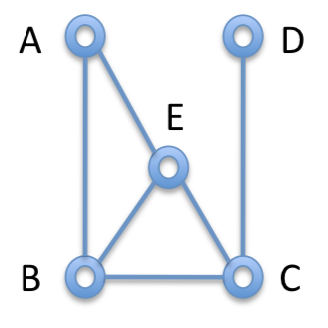
\includegraphics[width=0.2\textwidth,height=\textheight]{images/2.png}
\caption{Example 2}
\end{figure}

we can make several different spanning trees (two are below).

\begin{figure}
\centering
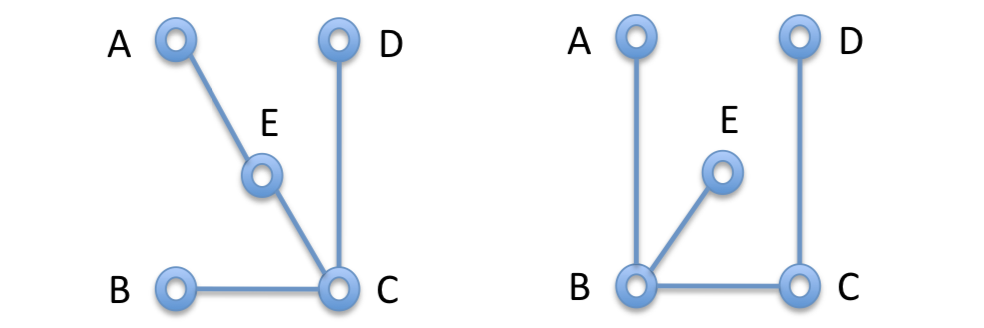
\includegraphics[width=0.5\textwidth,height=\textheight]{images/3.png}
\caption{Example 3}
\end{figure}

In general, one might ask how many different spanning trees exist for
any graph. The answer would be to use the \emph{Tutte Polynomial} (more
on that here \url{http://mathworld.wolfram.com/TuttePolynomial.html}).

For more on spanning trees, see
\url{https://www.cs.cmu.edu/~fp/courses/15122-f10/lectures/24-spanning.pdf}.

\hypertarget{minimum-spanning-trees-mst}{%
\subsection{Minimum Spanning Trees
(MST)}\label{minimum-spanning-trees-mst}}

\begin{itemize}
\tightlist
\item
  \emph{Minimum Spanning Tree (MST)}: a spanning tree with the minimum
  possible total edge weight
\end{itemize}

\begin{figure}
\centering
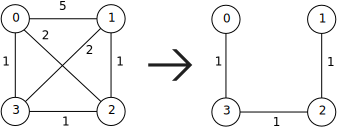
\includegraphics[width=0.5\textwidth,height=\textheight]{images/4.svg}
\caption{Example 4}
\end{figure}

\hypertarget{mst-algorithms}{%
\subsubsection{MST Algorithms}\label{mst-algorithms}}

\begin{itemize}
\tightlist
\item
  Idea: identify which edges should be included such that

  \begin{itemize}
  \tightlist
  \item
    All nodes are connected
  \item
    No cycle is formed
  \item
    Total weight is minimized
  \end{itemize}
\item
  Kruskal's Algorithm (use a priority queue and or heap)

  \begin{itemize}
  \tightlist
  \item
    Sort edges based on their weights in ascending order
  \item
    For each step, pick the lowest weighted one to add to the tree \(T\)
    unless it would create a cycle
  \end{itemize}
\item
  Prim's Algorithm (use a disjoint set)

  \begin{itemize}
  \tightlist
  \item
    Start with any vertex \(S\) and greedily grow a tree \(T\) from
    \(S\)
  \item
    For each step, pick the minimum edges that connects the current
    \(T\) and \((G-T)\)

    \begin{itemize}
    \tightlist
    \item
      Don't confuse this algorithm with Dijkstra's!
    \end{itemize}
  \end{itemize}
\item
  Both Kruskal's and Prim's algorithms are greedy

  \begin{itemize}
  \tightlist
  \item
    That means that they make locally optimal choices at each stage,
    with the intent of finding a global optimum (note: not \emph{the}
    global optimum, \emph{a} global optimum*)
  \item
    In many problems, a greedy strategy does not produce an optimal
    solution
  \end{itemize}
\item
  There are lots of other MST algorithms

  \begin{itemize}
  \tightlist
  \item
    \url{https://en.wikipedia.org/wiki/Minimum_spanning_tree}
  \end{itemize}
\end{itemize}

\hypertarget{summary}{%
\subsection{Summary}\label{summary}}

\begin{itemize}
\tightlist
\item
  Graphs

  \begin{itemize}
  \tightlist
  \item
    Basic definitions and terms
  \end{itemize}
\item
  Graph representation

  \begin{itemize}
  \tightlist
  \item
    Adjacency matrix and adjacency list
  \end{itemize}
\item
  Graph algorithms

  \begin{itemize}
  \tightlist
  \item
    Graph traversals
  \item
    Shortest path problem
  \item
    MST problem
  \end{itemize}
\end{itemize}

\hypertarget{next-lecture}{%
\subsection{Next Lecture}\label{next-lecture}}

\begin{itemize}
\tightlist
\item
  Priority queues

  \begin{itemize}
  \tightlist
  \item
    Reading: Chapter 6.9, Chapter 21
  \end{itemize}
\end{itemize}

\end{document}
